%%%%%%%%------------------------------------------------------------------------
% This program is free software: you can redistribute it and/or modify
% it under the terms of the GNU General Public License as published by
% the Free Software Foundation, either version 3 of the License, or
% (at your option) any later version.
% 
% This program is distributed in the hope that it will be useful,
% but WITHOUT ANY WARRANTY; without even the implied warranty of
% MERCHANTABILITY or FITNESS FOR A PARTICULAR PURPOSE.  See the
% GNU General Public License for more details.
% 
% You should have received a copy of the GNU General Public License
% along with this program.  If not, see <http://www.gnu.org/licenses/>.
%%%%%%%%------------------------------------------------------------------------
% Name:         xecjk-template
% Author:       Xiao Hanyu
% Email:        xiaohanyu1988@gmail.com
% Homepage:     http://cnlox.is-programmer.com
% Project Page: http://code.google.com/p/xecjk-template/
%               This is an xelatex template with xeCJK support. 
%%%%%%%%------------------------------------------------------------------------

%%%%%%%%------------------------------------------------------------------------
%%%% 导言区
%% 设定纸张大小为A4, 基本字体大小为12pt, 文章题目单独为一页, 
%% 文档类型为article
\documentclass[a4paper, 12pt, titlepage]{article}

%% en_preamble包含基本的宏包配置
%%%%%%%%------------------------------------------------------------------------
%%%% 日常所用宏包

%% 控制页边距
\usepackage[top=2.5cm, bottom=2.5cm, left=2.5cm, right=2.5cm]{geometry}

%% 控制项目列表
\usepackage{enumerate}

%% 多栏显示
\usepackage{multicol}

%% hyperref宏包,生成可定位点击的超链接,并且会生成pdf书签
\usepackage[%
    pdfstartview=FitH,%
    CJKbookmarks=true,%
    bookmarks=true,%
    bookmarksnumbered=true,%
    bookmarksopen=true,%
    colorlinks=true,%
    citecolor=blue,%
    linkcolor=blue,%
    anchorcolor=green,%
    urlcolor=blue%
]{hyperref}

%% 控制标题
\usepackage{titlesec}

%% 控制表格样式
\usepackage{booktabs}

%% 控制目录
\usepackage{titletoc}

%% 控制字体大小
\usepackage{type1cm}

%% 首行缩进,用\noindent取消某段缩进
\usepackage{indentfirst}

%% 支持彩色文本、底色、文本框等
\usepackage{color,xcolor}

%% AMS LaTeX宏包
\usepackage{amsmath}

%% 一些特殊符号
% \usepackage{bbding}

%% 支持引用
% \usepackage{cite}

%% LaTeX一些特殊符号宏包
% \usepackage{latexsym}

%% 数学公式中的黑斜体
% \usepackage{bm}

%% 调整公式字体大小:\mathsmaller, \mathlarger
% \usepackage{relsize}

%% 生成索引
% \makeindex

%%%% 基本插图方法
%% 图形宏包
\usepackage{graphicx}

%% 多个图形并排,参加lnotes.pdf
\usepackage{subfig}

% \begin{figure}[htbp]               %% 控制插图位置
%   \setlength{\abovecaptionskip}{0pt}
%   \setlength{\belowcaptionskip}{10pt}
                                     %% 控制图形和上下文的距离
%   \centering                       %% 使图形居中显示
%   \includegraphics[width=0.8\textwidth]{CTeXLive2008.jpg}
                                     %% 控制图形显示宽度为0.8\textwidth
%   \caption{CTeXLive2008安装过程} \label{fig:CTeXLive2008}
                                     %% 图形题目和交叉引用标签
% \end{figure}
%%%% 基本插图方法结束

%%%% pgf/tikz绘图宏包设置
\usepackage{pgf,tikz}
\usetikzlibrary{shapes,automata,snakes,backgrounds,arrows}
\usetikzlibrary{mindmap}
%% 可以直接在latex文档中使用graphviz/dot语言,
%% 也可以用dot2tex工具将dot文件转换成tex文件再include进来
%% \usepackage[shell,pgf,outputdir={docgraphs/}]{dot2texi}
%%%% pgf/tikz设置结束


%%%% fancyhdr设置页眉页脚
%% 页眉页脚宏包
\usepackage{fancyhdr}

%% 页眉页脚风格
\pagestyle{plain}

%% 有时会出现\headheight too small的warning
\setlength{\headheight}{15pt}

%% 清空当前页眉页脚的默认设置
%\fancyhf{}
%%%% fancyhdr设置结束


%%%% 设置listings宏包用来粘贴源代码
%% 方便粘贴源代码,部分代码高亮功能
\usepackage{listings}

%% 所要粘贴代码的编程语言
\lstloadlanguages{}

%% 设置listings宏包的一些全局样式
%% 参考http://hi.baidu.com/shawpinlee/blog/item/9ec431cbae28e41cbe09e6e4.html
\lstset{
showstringspaces=false,              %% 设定是否显示代码之间的空格符号
numbers=left,                        %% 在左边显示行号
numberstyle=\tiny,                   %% 设定行号字体的大小
basicstyle=\tiny,                    %% 设定字体大小\tiny, \small, \Large等等
keywordstyle=\color{blue!70}, commentstyle=\color{red!50!green!50!blue!50},
                                     %% 关键字高亮
frame=shadowbox,                     %% 给代码加框
rulesepcolor=\color{red!20!green!20!blue!20},
escapechar=`,                        %% 中文逃逸字符,用于中英混排
xleftmargin=2em,xrightmargin=2em, aboveskip=1em,
breaklines,                          %% 这条命令可以让LaTeX自动将长的代码行换行排版
extendedchars=false                  %% 这一条命令可以解决代码跨页时,章节标题,页眉等汉字不显示的问题
}
%%%% listings宏包设置结束


%%%% 附录设置
\usepackage[title,titletoc,header]{appendix}
%%%% 附录设置结束


%%%% 日常宏包设置结束
%%%%%%%%------------------------------------------------------------------------

%%%%%%%%------------------------------------------------------------------------
%%%% 英文字体设置结束
%% 这里可以加入自己的英文字体设置
%%%%%%%%------------------------------------------------------------------------

%%%%%%%%------------------------------------------------------------------------
%%%% 设置常用字体字号,与MS Word相对应

%% 一号, 1.4倍行距
\newcommand{\yihao}{\fontsize{26pt}{36pt}\selectfont}
%% 二号, 1.25倍行距
\newcommand{\erhao}{\fontsize{22pt}{28pt}\selectfont}
%% 小二, 单倍行距
\newcommand{\xiaoer}{\fontsize{18pt}{18pt}\selectfont}
%% 三号, 1.5倍行距
\newcommand{\sanhao}{\fontsize{16pt}{24pt}\selectfont}
%% 小三, 1.5倍行距
\newcommand{\xiaosan}{\fontsize{15pt}{22pt}\selectfont}
%% 四号, 1.5倍行距
\newcommand{\sihao}{\fontsize{14pt}{21pt}\selectfont}
%% 半四, 1.5倍行距
\newcommand{\bansi}{\fontsize{13pt}{19.5pt}\selectfont}
%% 小四, 1.5倍行距
\newcommand{\xiaosi}{\fontsize{12pt}{18pt}\selectfont}
%% 大五, 单倍行距
\newcommand{\dawu}{\fontsize{11pt}{11pt}\selectfont}
%% 五号, 单倍行距
\newcommand{\wuhao}{\fontsize{10.5pt}{10.5pt}\selectfont}
%%%%%%%%------------------------------------------------------------------------


%%%%%%%%------------------------------------------------------------------------
%%%% 一些个性设置

%% 设定页码方式,包括arabic、roman等方式
%% \pagenumbering{arabic}

%% 有时LaTeX无从断行,产生overfull的错误,这条命令降低LaTeX断行标准
%% \sloppy

%% 设定段间距
\setlength{\parskip}{0.5\baselineskip}

%% 设定行距
\linespread{1}

%% 中文破折号,据说来自清华模板
\newcommand{\pozhehao}{\kern0.3ex\rule[0.8ex]{2em}{0.1ex}\kern0.3ex}

%% 设定itemize环境item的符号
\renewcommand{\labelitemi}{$\bullet$}

%% 设定正文字体大小
% \renewcommand{\normalsize}{\sihao}

%%%% 个性设置结束
%%%%%%%%------------------------------------------------------------------------


%%%%%%%%------------------------------------------------------------------------
%%%% bibtex设置

%% 设定参考文献显示风格
\bibliographystyle{plain}

%%%% bibtex设置结束
%%%%%%%%------------------------------------------------------------------------


%% 如果不写中文的话就不需要引用xecjk_preamble里面的配置
%%%%%%%%------------------------------------------------------------------------
%%%% xeCJK相关宏包

\usepackage{xltxtra,fontspec,xunicode}

%% \CJKsetecglue{\hskip 0.15em plus 0.05em minus 0.05em}
%% slanfont: 允许斜体
%% boldfont: 允许粗体
%% CJKnormalspaces: 仅忽略汉字之间的空白,但保留中英文之间的空白。 
%% CJKchecksingle: 避免单个汉字单独占一行。
\usepackage[slantfont, boldfont]{xeCJK} 

%% 针对中文进行断行
\XeTeXlinebreaklocale "zh"             

%% 给予TeX断行一定自由度
\XeTeXlinebreakskip = 0pt plus 1pt minus 0.1pt

%%%% xeCJK设置结束                                       
%%%%%%%%------------------------------------------------------------------------

%%%%%%%%------------------------------------------------------------------------
%%%% xeCJK字体设置

%% 设置中文标点样式,支持quanjiao、banjiao、kaiming等多种方式
\punctstyle{kaiming}                                        
                                                     
%% 设置缺省中文字体
\setCJKmainfont[BoldFont={Adobe Heiti Std}, ItalicFont={Adobe Kaiti Std}]{Adobe Song Std}   
%% 设置中文无衬线字体
\setCJKsansfont[BoldFont={Adobe Heiti Std}]{Adobe Kaiti Std}  
%% 设置等宽字体
\setCJKmonofont{Adobe Heiti Std}                            

%% 英文衬线字体
\setmainfont{DejaVu Serif}                                  
%% 英文等宽字体
\setmonofont{DejaVu Sans Mono}                              
%% 英文无衬线字体
\setsansfont{DejaVu Sans}                                   

%% 定义新字体
\setCJKfamilyfont{song}{Adobe Song Std}                     
\setCJKfamilyfont{kai}{Adobe Kaiti Std}
\setCJKfamilyfont{hei}{Adobe Heiti Std}
\setCJKfamilyfont{fangsong}{Adobe Fangsong Std}
\setCJKfamilyfont{lisu}{LiSu}
\setCJKfamilyfont{youyuan}{YouYuan}

%% 自定义宋体
\newcommand{\song}{\CJKfamily{song}}                       
%% 自定义楷体
\newcommand{\kai}{\CJKfamily{kai}}                         
%% 自定义黑体
\newcommand{\hei}{\CJKfamily{hei}}                         
%% 自定义仿宋体
\newcommand{\fangsong}{\CJKfamily{fangsong}}               
%% 自定义隶书
\newcommand{\lisu}{\CJKfamily{lisu}}                       
%% 自定义幼圆
\newcommand{\youyuan}{\CJKfamily{youyuan}}                 

%%%% xeCJK字体设置结束
%%%%%%%%------------------------------------------------------------------------

%%%%%%%%------------------------------------------------------------------------
%%%% 一些关于中文文档的重定义

%% 数学公式定理的重定义

\newtheorem{example}{例}                                   
\newtheorem{algorithm}{算法}
%% 按section编号
\newtheorem{theorem}{定理}[section]                         
\newtheorem{definition}{定义}
\newtheorem{axiom}{公理}
\newtheorem{property}{性质}
\newtheorem{proposition}{命题}
\newtheorem{lemma}{引理}
\newtheorem{corollary}{推论}
\newtheorem{remark}{注解}
\newtheorem{condition}{条件}
\newtheorem{conclusion}{结论}
\newtheorem{assumption}{假设}

%% 章节等名称重定义
\renewcommand{\contentsname}{目录}     
\renewcommand{\abstractname}{摘要}
\renewcommand{\indexname}{索引}
\renewcommand{\listfigurename}{插图目录}
\renewcommand{\listtablename}{表格目录}
\renewcommand{\figurename}{图}
\renewcommand{\tablename}{表}
\renewcommand{\appendixname}{附录}
\renewcommand{\appendixpagename}{附录}
\renewcommand{\appendixtocname}{附录}
\renewcommand\refname{参考文献} 

%% 设置chapter、section与subsection的格式
\titleformat{\chapter}{\centering\huge}{第\thechapter{}章}{1em}{\textbf}
\titleformat{\section}{\centering\sihao}{\thesection}{1em}{\textbf}
\titleformat{\subsection}{\xiaosi}{\thesubsection}{1em}{\textbf}
\titleformat{\subsubsection}{\xiaosi}{\thesubsubsection}{1em}{\textbf}

%%%% 中文重定义结束
%%%%%%%%------------------------------------------------------------------------


%%%% 导言区结束
%%%%%%%%------------------------------------------------------------------------

%%%%%%%%------------------------------------------------------------------------
%%%% 正文部分

\begin{document}

%% 中文习惯是设定首行缩进为2em。注意此设置一定要在document环境之中,这可能与\setlength作用范围相关
\setlength{\parindent}{2em}                    

\title{XeTeX and xeCJK sample template}
\author{Xiao Hanyu}
\maketitle


\tableofcontents
\listoffigures
\listoftables

\section{基本文字测试}
\label{sec:1}
我叫肖晗宇,来自浙江大学计算机学院,热爱开源软件、旅行、摄影,推崇互助共享的精神理念。

My name is Xiao Hanyu, a student from Computer Science and Technology of Zhejiang University, I love open source software, travelling all over the world, photography, and so on. 

我喜欢\LaTeXe,也推荐大家来学习使用\LaTeXe,以下是比较不错的学习资源:

\begin{enumerate}
\item LaTeX companion
\item The TeXbook
\end{enumerate}


\section{图形图像测试}
\subsection{插图测试}
Hand in Hand:\ref{fig:hand_in_hand}
\begin{figure}[htbp]
\centerline{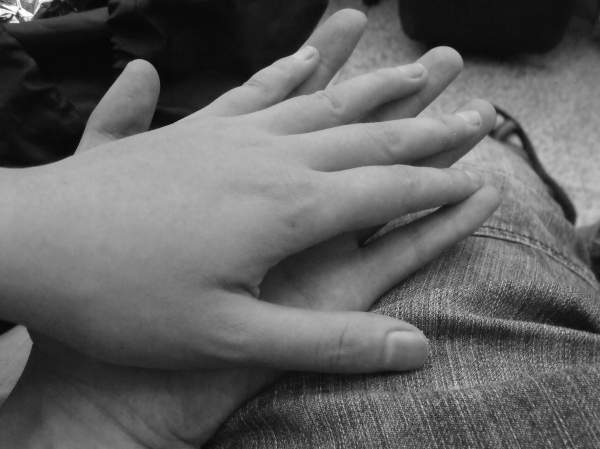
\includegraphics[width=0.6\textwidth]{images/hand_in_hand.png}}
\caption[]{\label{fig:hand_in_hand} 手拉手}
\end{figure}

\subsection{pgf/tikz绘图测试}
图\ref{fig:monotonic_chain}是用pgf/tikz宏包作的图形,用以说明计算几何相关定理。

\begin{figure}
\centering
\begin{tikzpicture}[line width=2pt]
\draw (-1,0) -- (8,0);
\draw (0,-1) -- (0,8);
\draw[step=.5cm, very thin] (0,0) grid (7.2,7.2);

\coordinate [label=above:$A$] (A) at (1, 4);
\coordinate [label=left:$B$] (B) at (0.5, 3.5);
\coordinate [label=left:$C$] (C) at (1, 3);
\coordinate [label=left:$D$] (D) at (0.3, 1.3);
\coordinate [label=below:$E$] (E) at (1, 1);

\draw[blue] (A) -- (B) -- (C)  -- (D) -- (E);
\draw[blue] (2, 0) -- (2, 6);

\coordinate [label=right:$A'$] (A') at (2, 4);
\coordinate [label=right:$B'$] (B') at (2, 3.5);
\coordinate [label=right:$C'$] (C') at (2, 3);
\coordinate [label=right:$D'$] (D') at (2, 1.3);
\coordinate [label=right:$E'$] (E') at (2, 1);

\draw[blue] (A) -- (A');
\draw[blue] (B) -- (B');
\draw[blue] (C) -- (C');
\draw[blue] (D) -- (D');
\draw[blue] (E) -- (E');

\coordinate [label=above:$a$] (a) at (5, 4);
\coordinate [label=left:$b$] (b) at (4.5, 4.5);
\coordinate [label=left:$c$] (c) at (5, 3);
\coordinate [label=left:$d$] (d) at (4.3, 1.3);
\coordinate [label=below:$e$] (e) at (5, 1.3);

\draw[green] (a) -- (b) -- (c)  -- (d) -- (e);
\draw[green] (6, 0) -- (6, 6);

\coordinate [label=right:$a'$] (a') at (6, 4);
\coordinate [label=right:$b'$] (b') at (6, 4.5);
\coordinate [label=right:$c'$] (c') at (6, 3);
\coordinate [label=right:$d'$] (d') at (6, 1.3);
\coordinate [label=right:$e'$] (e') at (6, 1.3);

\draw[green] (a) -- (a');
\draw[green] (b) -- (b');
\draw[green] (c) -- (c');
\draw[green] (d) -- (d');
\draw[green] (e) -- (e');
\end{tikzpicture}
\caption{Monotonic polygonal chains}
\label{fig:monotonic_chain}
\end{figure}

\section{表格测试}
\begin{table}[htbp]
  \centering
  \begin{tabular}[htbp]{r|l}
    \toprule
    日期 & 任务 \\
    \midrule
    2011.5 & 完善此份文档 \\
    2011.6 & 完善安装脚本 \\
    \bottomrule
  \end{tabular}
  \caption{表格}
  \label{tab:table1}
\end{table}

\section{源代码高亮测试}

以下是\href{http://acm.zju.edu.cn/onlinejudge/showProblem.do?problemCode=1372}{ZOJ 1372}的解题c++代码:

\begin{lstlisting}[language=c++]
#include <iostream>
#include <string>
using namespace std;
 
const long max_points = 100;
const long infinity = 1000001;
 
int p, r, length, g[max_points][max_points];
bool flag;
 
class vertex
{
public:
    int distance;
    bool visited;
};
 
vertex v[max_points];
 
void initial()
{
    for(int i = 1; i <= p; i++)
        for(int j = 1; j <= p; j++)
            g[i][j] = infinity;
}
 
void prim(int origin)
{
    int temp_min;
    int temp_v = 0;
    int sum = 0;
 
    for(int i = 1; i <= p; i++)
    {
        v[i].distance = g[i][origin];
        v[i].visited = false;
    }
 
    v[origin].distance = 0;
    v[origin].visited = true;
 
    sum++;
 
    while (sum < p)
    {
        temp_min = infinity;
        for(int i = 1; i <= p; i++)
            if(v[i].visited == false && v[i].distance < temp_min)
            {
                temp_min = v[i].distance;
                temp_v = i;
            }
         
        if(temp_min < infinity)
        {
            length += v[temp_v].distance;
            v[temp_v].visited = true;
            sum++;
        }
        else
        {
            flag = true;
            break;
        }
 
        for(int i = 1; i <= p; i++)
        {
            if(v[i].visited == false && v[i].distance > g[i][temp_v])
            {
                v[i].distance = g[i][temp_v];
            }
        }
    }
}
 
int main(int argc, char *argv[])
{
    int a, b, c;
 
    while(cin >> p)
    {
        if(p == 0)
            break;
        cin >> r;
 
        initial();
 
        for(int i = 0; i < r; i++)
        {
            cin >> a >> b >> c;
            if(c < g[a][b])
                g[a][b] = g[b][a] = c;
        }
        length = 0;
        prim(1);
 
        cout << length << endl;
    }
 
    return 0;
} 
\end{lstlisting}

\section{数学公式测试}

著名的爱因斯坦质能方程(\ref{eq:emc2}):

\begin{equation}
  \label{eq:emc2}
  E=mc^2
\end{equation}

计算$f(x)=x^2$的不定积分(\ref{eq:2}):

\begin{equation}
  \label{eq:2}
  \int x^2 dx = \frac{1}{3} x^3
\end{equation}
%%%%%%%%------------------------------------------------------------------------
%%%% 附录

% \appendix    
% \appendixpage
%% 将附录条目添加到contents
% \addappheadtotoc

%%%% 附录结束
%%%%%%%%------------------------------------------------------------------------

\bibliography{main}                    % 加入参考文献,需要bibtex支持

\end{document}
%%%% 正文部分结束
%%%%%%%%------------------------------------------------------------------------
